%
% section 3.2
%
\section{Το Αυτοδύναμο Πακέτο IP (Datagram) -- Δομή Πακέτου}

Το \emph{πρωτόκολλο διαδικτύου (Internet Protocol -- IP)} ενθυλακώνει τα πακέτα δεδομένων που του προωθούνται από ανώτερο επίπεδο (μεταφοράς) σε \emph{αυτοδύναμα πακέτα (datagrams)}. Τυπικά, το επίπεδο μεταφοράς προωθεί είτε τμήματα TCP (TCP Segments) είτε αυτοδύναμα πακέτα UDP (UDP Datagrams) και θα τα εξετάσουμε σε επόμενο κεφάλαιο. Το IP προσθέτει στη δική του επικεφαλίδα πεδία που περιέχουν όλες τις απαραίτητες διαχειριστικές πληροφορίες ώστε να γίνει δυνατή η εύρεση του προορισμού και η επιτυχής δρομολόγηση του πακέτου από τα πρωτόκολλα δρομολόγησης.

Τα πιο σημαντικά πεδία είναι η \emph{Διεύθυνση IP Προέλευσης (Source IP)} και η \emph{Διεύθυνση IP Προορισμού (Destination IP)} με μήκος 32 bit η κάθε μία (στην έκδοση IPv4).

Μπορείτε να δείτε την δομή του πρωτοκόλλου IP στο σχήμα \ref{3-5}. Θα αναλύσουμε τα σημαντικότερα πεδία:

\begin{figure}[!ht]
  \centering
  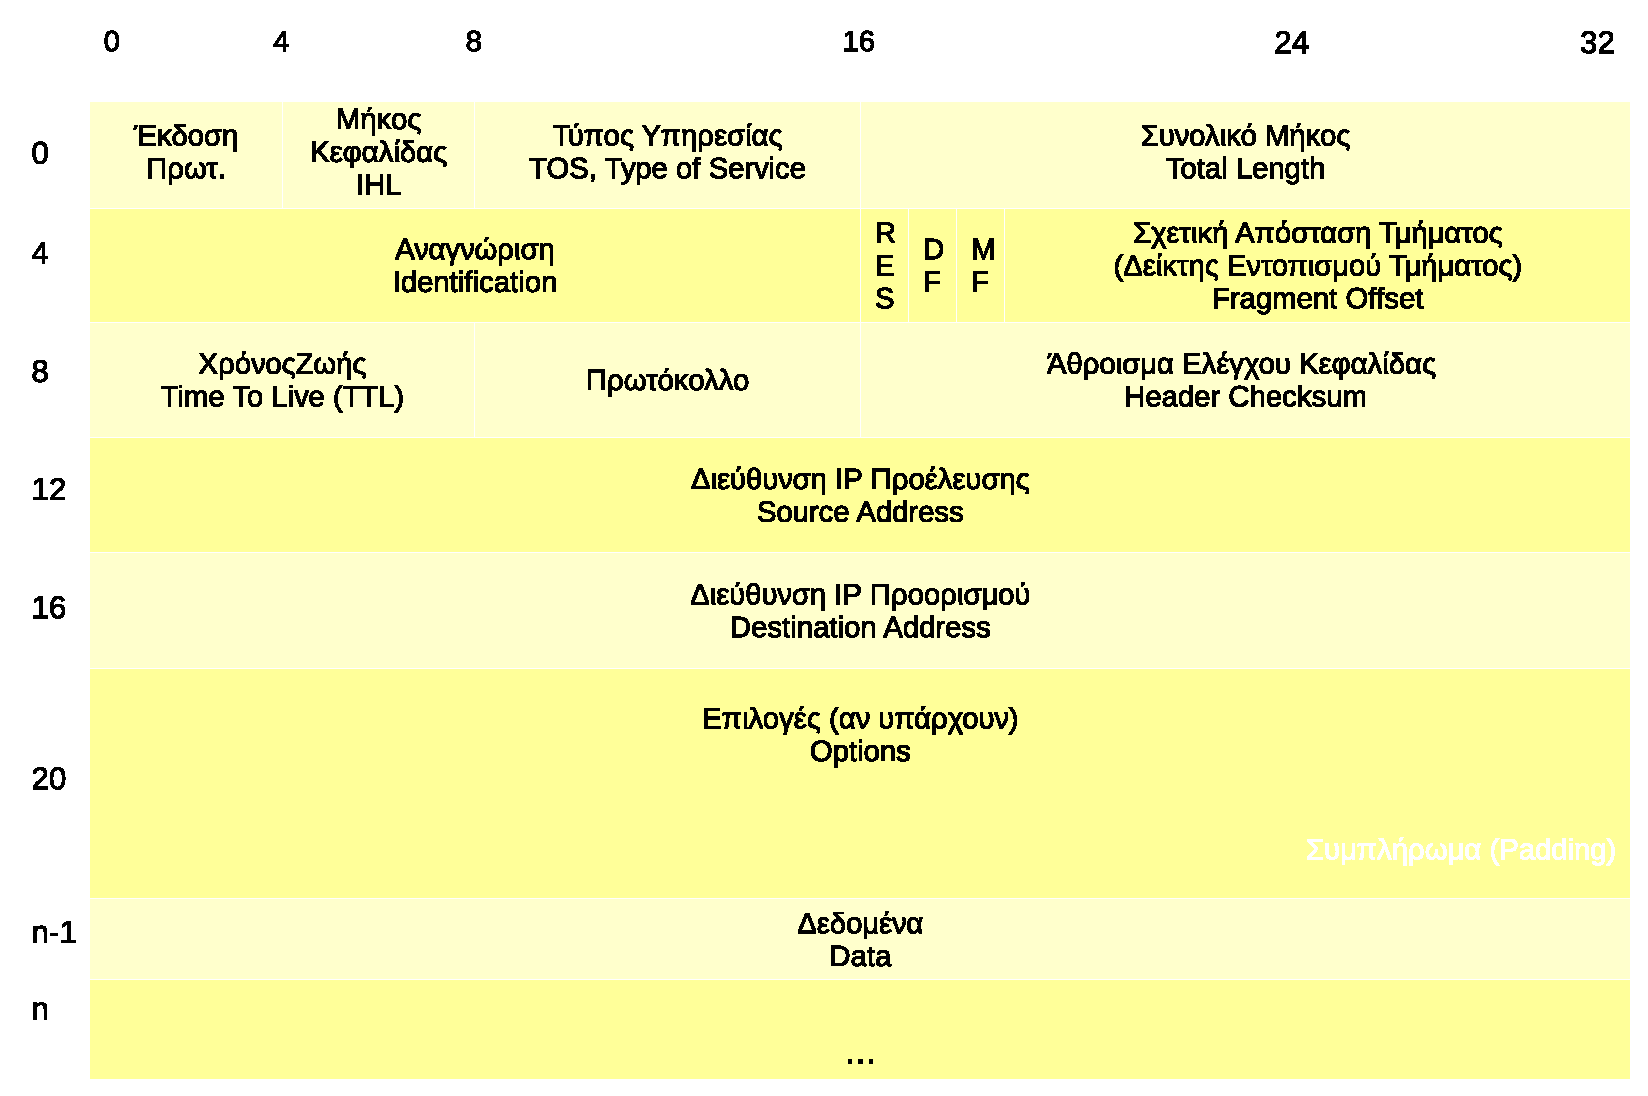
\includegraphics[width=0.95\textwidth]{images/chapter3/3-5}
  \caption {\textsl{Δομή Αυτοδύναμου Πακέτου IP}}
  \label{3-5}
\end{figure}

\begin{itemize}
\item \textbf{Έκδοση Πρωτοκόλλου:} Το πεδίο αυτό έχει μέγεθος 4 bit και δηλώνει την έκδοση του πρωτοκόλλου IP που χρησιμοποιείται. Έχει τις τιμές 4 για IPv4 και 6 για IPv6. Αν χρησιμοποιείται IPv6, η επικεφαλίδα έχει ελάχιστο μήκος 40 bytes.
\item \textbf{Μήκος Επικεφαλίδας:} Το πεδίο αυτό είναι μήκους 4 bit και εκφράζει το μήκος της επικεφαλίδας σε λέξεις των 32bit. Έτσι αν έχει τιμή 5, η επικεφαλίδα είναι 32Χ5=160 bit και άρα 160/8=20 bytes. Μπορείτε επίσης να πολλαπλασιάσετε την τιμή του πεδίου αυτού με το 4 για να βρείτε απευθείας το μήκος της επικεφαλίδας σε bytes.

\begin{inthebox}
\textbf{Προσέξτε} ότι στις ασκήσεις άλλες φορές δίνεται το μήκος της επικεφαλίδας σε bytes (π.χ. 20 bytes) και άλλες \textbf{η τιμή του πεδίου ``μήκος επικεφαλίδας''} οπότε πρέπει να πολλαπλασιάσουμε με το 4 για να βρούμε τα bytes της επικεφαλίδας.\\
\end{inthebox}

Το ελάχιστο μήκος επικεφαλίδας είναι 5 λέξεις των 32 bit ή 20 bytes και το μέγιστο 15 λέξεις ή 60 bytes (4X15).
\item \textbf{Τύπος Υπηρεσίας:} Το πεδίο αυτό έχει μήκος 8 bit και περιγράφει τον επιθυμητό χειρισμό του πακέτου από κάθε κόμβο που θα περάσει. Μπορεί να δίνεται προτεραιότητα στην ταχύτητα, εάν δηλ. επιτρέπεται να καθυστερήσει ή όχι, στην αξιοπιστία ή στο ρυθμό διακίνησης (throughput). Με νεώτερη αναθεώρηση, το RFC2474 αλλάζει τη σημασία του συγκεκριμένου πεδίου ώστε να υποστηρίζει ένα σύνολο διαφοροποιημένων υπηρεσιών που ονομάζει \emph{Differentiated Services Code Point - DSCP (6 bit)}. Τα υπόλοιπα 2 bit χαρακτηρίζονται από το RFC3168 ως ρητή ειδοποίηση συμφόρησης, \emph{Explicit Congestion Notification, ECN}. Οι αλλαγές αυτές έγιναν με σκοπό να υποστηρίξουν νέες υπηρεσίες με ιδιαίτερες απαιτήσεις όπως η μεταφορά φωνής μέσω VoIP. Για να είναι αυτό εφικτό πρέπει οι υπηρεσίες να υποστηρίζονται και από το υπόλοιπο δίκτυο. 

\item \textbf{Συνολικό Μήκος:} Το πεδίο αυτό έχει μέγεθος 16 bits και δηλώνει το συνολικό μήκος (επικεφαλίδα και δεδομένα) του πακέτου σε bytes. Η ελάχιστη τιμή που μπορεί να πάρει είναι 20 (αντιπροσωπεύει ένα πακέτο με μόνο το βασικό, σταθερό τμήμα της επικεφαλίδας χωρίς καθόλου δεδομένα) μέχρι 65535 (τιμή που αντιστοιχεί σε 16 άσους). Αυτό σημαίνει ότι το \emph{μέγιστο μέγεθος του αυτοδύναμου πακέτου IP} στο IPv4 είναι 65535 bytes (πρακτικά, 64 Kbyte).

\item \textbf{Αναγνώριση:} Καθώς το πακέτο IP κινείται προς τον προορισμό του, ενδέχεται να περάσει από αρκετά ενδιάμεσα δίκτυα.Το μέγιστο μήκος δεδομένων που μπορεί να μεταδοθεί σε ένα πλαίσιο από το επίπεδο ζεύξης δεδομένων ενός δικτύου είναι γνωστό με την ονομασία \emph{MTU, Maximum Transfer Unit}. Έτσι, για παράδειγμα το Ethernet έχει MTU 1500 bytes (κάθε πλαίσιο Ethernet μπορεί να μεταδώσει μέχρι 1500 bytes δεδομένων). Διαφορετικοί τύποι δικτύων έχουν άλλο MTU. Ένα πακέτο IP ενδέχεται να έχει μέγεθος τέτοιο που να μην μπορεί να μεταδοθεί από ένα ενδιάμεσο δίκτυο χωρίς να διασπαστεί περισσότερο. 

Στην περίπτωση αυτή, αν το πακέτο επιτρέπεται να διασπαστεί, θα χωριστεί σε τμήματα που ονομάζονται \emph{fragments}. Η διαδικασία είναι γνωστή ως \emph{διάσπαση ή κατάτμηση (IP Fragmentation)}. Όταν τα τμήματα φτάσουν στο προορισμό τους θα πρέπει να επανασυνδεθούν για να σχηματίσουν ξανά το αρχικό πακέτο IP. Καθώς στον παραλήπτη μπορεί να φτάνουν τμήματα από πακέτα IP που προέρχονται από διαφορετικές επικοινωνίες, το πεδίο \emph{Αναγνώριση} περιέχει ένα αριθμό που χρησιμοποιείται για να αναγνωριστούν ποια τμήματα ανήκουν σε κάθε πακέτο: όλα τα τμήματα που προέρχονται από τη διάσπαση ενός συγκεκριμένου πακέτου έχουν τον ίδιο αριθμό αναγνώρισης.

\item \textbf{Σχετική Θέση Τμήματος ή Δείκτης Εντοπισμού Τμήματος:} Και αυτό το πεδίο (όπως και η Αναγνώριση) χρησιμοποιείται στην περίπτωση που έχουμε διάσπαση. Χρησιμοποιείται για να μπουν ξανά τα fragments στη σωστή σειρά στον υπολογιστή προορισμού. Το πεδίο έχει μέγεθος 13 bits και ο αριθμός που περιέχει εκφράζει την απόσταση του τμήματος από το πρώτο σε οκτάδες (8x) byte. Η σχετική θέση τμήματος είναι πάντοτε μηδέν στο πρώτο τμήμα. Στα επόμενα τμήματα, την υπολογίζουμε διαιρώντας τα καθαρά δεδομένα (χωρίς επικεφαλίδα) που έχουν μεταδοθεί μέχρι εκείνη τη στιγμή  με το οκτώ.

Για παράδειγμα, αν διασπάσουμε ένα πακέτο συνολικού μήκους 1500 bytes σε δίκτυο με MTU 500 bytes:

\begin{itemize}
\item Τα δεδομένα του αρχικού πακέτου είναι 1500 bytes - 20 bytes επικεφαλίδα = 1480 bytes
\item Το πρώτο τμήμα θα έχει Σχετική Θέση Τμήματος μηδέν και συνολικό μήκος 500 bytes. Από αυτά, τα 20 είναι επικεφαλίδα. Συνολικά θα μεταδώσουμε 480 bytes καθαρών δεδομένων.
\item Το δεύτερο τμήμα θα έχει Σχετική Θέση Τμήματος 480/8 = 60 και θα είναι επίσης 500 bytes συνολικό μήκος. Θα περιέχει επίσης 480 bytes δεδομένων.
\item Το τρίτο τμήμα θα έχει Σχετική Θέση Τμήματος 960/8 = 120 (ή 2Χ60) και συνολικό μήκος 500 bytes. Θα περιέχει 480 bytes δεδομένων.
\item Για το τέταρτο και τελευταίο τμήμα έχουν μείνει 40 bytes δεδομένων, αφού έχουμε ήδη μεταδώσει 3Χ480=1440 bytes. Το συνολικό μήκος είναι 60 bytes και η Σχετική Θέση Τμήματος είναι 1440/8=180 (ή 3Χ60).
\end{itemize}   

\end{itemize}



 